\documentclass[a4paper,14pt]{extarticle}

\usepackage{cmap}
\usepackage[T2A]{fontenc}
\usepackage[utf8x]{inputenc}
\usepackage[english, russian]{babel}

\usepackage{misccorr} % в заголовках появляется точка, но при ссылке на них ее нет
\usepackage{amssymb,amsfonts,amsmath,amsthm}  
\usepackage{indentfirst}
\usepackage[usenames,dvipsnames]{color} 
\usepackage[unicode,hidelinks]{hyperref}
% \hypersetup{%
%     pdfborder = {0 0 0}
% }

\usepackage{makecell,multirow} 
\usepackage{ulem}
\usepackage{graphicx,wrapfig}
\graphicspath{{img/}}
\usepackage{geometry}
\geometry{left=2cm,right=2cm,top=3cm,bottom=3cm,bindingoffset=0cm,headheight=15pt}
\usepackage{fancyhdr} 
\linespread{1.05} 
\frenchspacing 
\renewcommand{\labelenumii}{\theenumii)} 
\newcommand{\mean}[1]{\langle#1\rangle}
% \usepackage{caption}
%%%%%%%%%%%%%%%%%%%%%%%%%%%%%%%%%%%%%%%%%%%%%%%%%%%%%%%%%%%%%%%%%%%%%%%%%%%%%%%
%%%%%%%%%%%%%%%%%%%%%%%%%%%%%%%%%%%%%%%%%%%%%%%%%%%%%%%%%%%%%%%%%%%%%%%%%%%%%%%

\def\labauthors{Есюнин Д.В., Есюнин М.В.}
\def\labgroup{440}
% \def\department{Кафедра электроники и квантовой физики}
\def\labnumber{1}
\def\labtheme{Замедляющие системы типа гребенки}

%%%%%%%%%%%%%%%%%%%%%%%%%%%%%%%%%%%%%%%%%%%%%%%%%%%%%%%%%%%%%%%%%%%%%%%%%%%%%%%
	%применим колонтитул к стилю страницы
\pagestyle{fancy} 
	%очистим "шапку" страницы
\fancyhead{} 
	%слева сверху на четных и справа на нечетных
\fancyhead[L]{\labauthors} 
	%справа сверху на четных и слева на нечетных
%\fancyhead[R]{Отчёт по лабораторной работе №\labnumber} 
	%очистим "подвал" страницы
\fancyfoot{} 
	% номер страницы в нижнем колинтуле в центре
\fancyfoot[C]{\thepage} 
\renewcommand{\phi}{\varphi}
%%%%%%%%%%%%%%%%%%%%%%%%%%%%%%%%%%%%%%%%%%%%%%%%%%%%%%%%%%%%%%%%%%%%%%%%%%%%%%%

\usepackage{float}
\usepackage[mode=buildnew]{standalone}
\usepackage{tikz} 
% \usepackage{subcaption}
\usepackage{tikz,csvsimple}
\usetikzlibrary{scopes}
\usetikzlibrary{%
     decorations.pathreplacing,%
     decorations.pathmorphing,%
    patterns,%
    calc,%
    scopes,%
    arrows,%
    % arrows.spaced,%
}
\makeatletter
\newif\if@gather@prefix 
\preto\place@tag@gather{% 
  \if@gather@prefix\iftagsleft@ 
    \kern-\gdisplaywidth@ 
    \rlap{\gather@prefix}% 
    \kern\gdisplaywidth@ 
  \fi\fi 
} 
\appto\place@tag@gather{% 
  \if@gather@prefix\iftagsleft@\else 
    \kern-\displaywidth 
    \rlap{\gather@prefix}% 
    \kern\displaywidth 
  \fi\fi 
  \global\@gather@prefixfalse 
} 
\preto\place@tag{% 
  \if@gather@prefix\iftagsleft@ 
    \kern-\gdisplaywidth@ 
    \rlap{\gather@prefix}% 
    \kern\displaywidth@ 
  \fi\fi 
} 
\appto\place@tag{% 
  \if@gather@prefix\iftagsleft@\else 
    \kern-\displaywidth 
    \rlap{\gather@prefix}% 
    \kern\displaywidth 
  \fi\fi 
  \global\@gather@prefixfalse 
} 
\newcommand*{\beforetext}[1]{% 
  \ifmeasuring@\else
  \gdef\gather@prefix{#1}% 
  \global\@gather@prefixtrue 
  \fi
} 
\makeatother

\usepackage{booktabs}
\usepackage{pgfplots, pgfplotstable}

\usepackage[outline]{contour}
\usepackage{tocloft}
\renewcommand{\cftsecleader}{\cftdotfill{\cftdotsep}} % for parts
% \renewcommand{\cftchapleader}{\cftdotfill{\cftdotsep}} % for chapters
\usepackage{pgfplots,pgfplotstable,booktabs,colortbl}
\pgfplotsset{compat=newest}
\usepackage{physics}
\usepackage{mathtools}
\mathtoolsset{showonlyrefs=true}
\newcommand\Smat{\hat { \mathbf { S } }}

\newcommand*\dotvec[1][1,1]{\crossproducttemp#1\relax}
\def\crossproducttemp#1,#2\relax{{\qty[\vec{#1}\times\vec{#2}\,]}}

\newcommand*\prodvec[1][1,1]{\crossproducttempa#1\relax}
\def\crossproducttempa#1,#2\relax{{\qty[{#1}\times{#2}\,]}}

% \def\E{\mathscr{E}_H}
\def\Rdim{\,\frac{\text{м}^3}{\text{А} \cdot \text{с}}}

\renewcommand{\vec}{\mathbf} % for parts


\begin{document}
	\begin{titlepage}

		\begin{center}
			
			
			\textsc{Нижегородский государственный университет имени Н.\,И. Лобачевского}
			\vskip 4pt \hrule \vskip 8pt
			\textsc{Радиофизический факультет}
			
			\vfill
			
			{\Large\labtheme}
			
		\end{center}
		
		\vfill
		
		\begin{flushright}
			{Работу выполнили студенты\\ \labauthors\\ 440 группы}
		\end{flushright}
		
		\vfill
		
		\begin{center}
			Нижний Новгород, \the\year
		\end{center}
	\end{titlepage}
%	\tableofcontents
	\newpage 
Цель работы: изучение волн, направляемых замедляющими системами типа гребенки рис.\ref{pic1}.
	\begin{figure}[H]
		\centering
		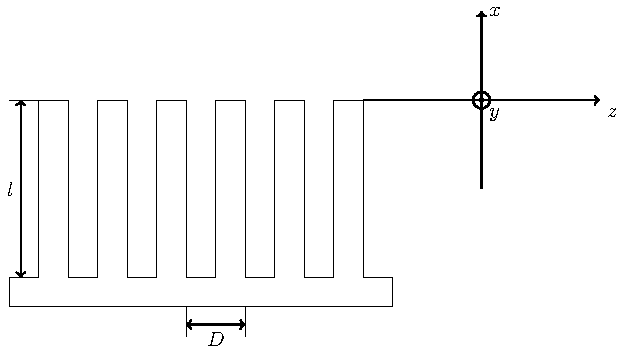
\includegraphics[width=\linewidth]{plots/pic1}
		\caption{Замедляющая система типа гребенки}
		\label{pic1}
	\end{figure}
\section*{Измерительная установка}
Измерительная установка включает генератор с диапазоном изменения частоты 2000-4000 МГц, два вентиля, две измерительные линии с вмонтированными в них гребенками, отличающимися высотой зубьев: $l_1= 8 мм$, $l_2= 22 мм$, и два амперметра. блок-схема установки представлена на рис.\ref{pic2}. Вентиль пропускает сигнал, идущий от генератора к замедляющей системе, и не пропускает сигнал, отраженный от замедляющей системы, к генератору. Тем самым исключается влияние нагрузки на работу генератора. По скольку линия закорочена на конце, в ней формируется стоячая волна. Регулировочный винт позволяет поднимать или опускать гребенку и тем самым изменяет положение относительно крышки.
\begin{figure}[H]
	\centering
	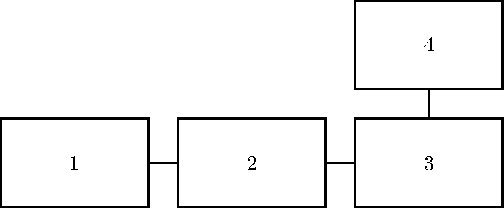
\includegraphics[width=0.7\linewidth]{plots/pic2}
	\caption{Блок-схема установки: }
	\label{pic2}
\end{figure}
{\centering 1 - генератор; 2 - вентиль; 3 - измерительная линия; 4 - амперметр}
\section*{Практическая часть}
\subsection*{Задание 1}
Сняли дисперсионные характеристики гребенок 1 и 2; результаты представили в виде графиков.

\begin{table}[htbp]
	\centering
	\caption{гребенка 1, $l_1 =22 \text{мм}$}
	\begin{tabular}{|l|r|r|r|r|r|r|r|r|r|r|r|}
		\hline
		$\nu, \text{ГГц}$ & 2     & 2.1   & 2.2   & 2.3   & 2.4   & 2.5   & 2.6   & 2.7   & 2.8   & 2.9   & 3 \\
		\hline
		$h, \text{см}^{-1}$ & 0.67  & 0.70  & 0.79  & 0.87  & 0.98  & 1.01  & 1.16  & 1.37  & 1.50  & 1.96  & 2.86 \\
		\hline
	\end{tabular}%
	\label{tab:addlabel}%
\end{table}%

% Table generated by Excel2LaTeX from sheet 'Лист1'
\begin{table}[htbp]
	\centering
	\caption{гребенка 2, $l_2 =8 \text{мм}$}
	\begin{tabular}{|l|r|r|r|r|r|r|r|r|r|}
		\hline
		$\nu, \text{ГГц}$ & 1.92  & 2.15  & 2.23  & 2.38  & 2.53  & 2.73  & 2.95  & 3.32  & 3.64 \\
		\hline
		$h, \text{см}^{-1}$ & 0.37  & 0.84  & 0.68  & 0.64  & 0.70  & 0.52  & 0.72  & 0.79  & 1.14 \\
		\hline
	\end{tabular}%
	\label{tab:addlabel}%
\end{table}%

\begin{figure}[H]
	\centering
	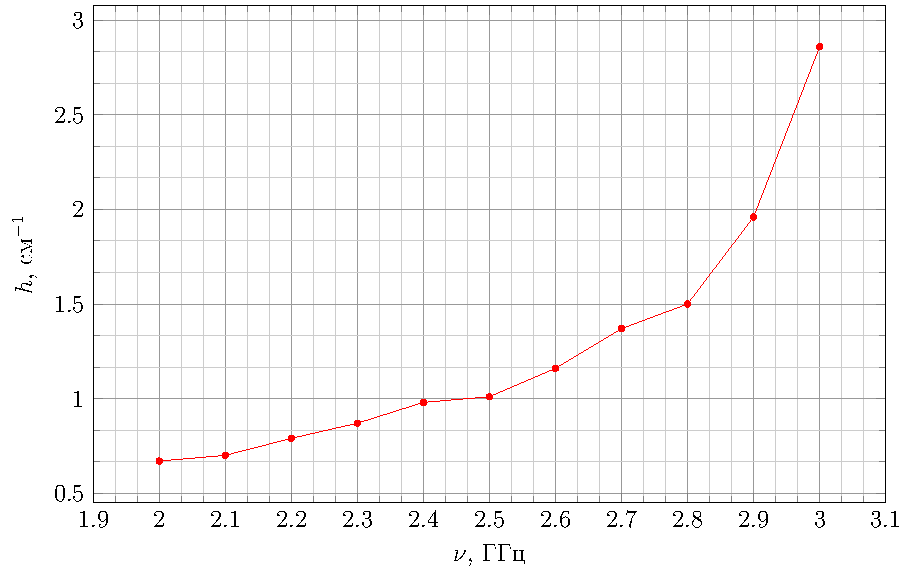
\includegraphics[width=0.8\linewidth]{plots/task1_1}
	\caption{дисперсионная характеристика гребенки 1 $l_1=22 \text{мм}$}
	\label{task1_1}
\end{figure}
\begin{figure}[H]
	\centering
	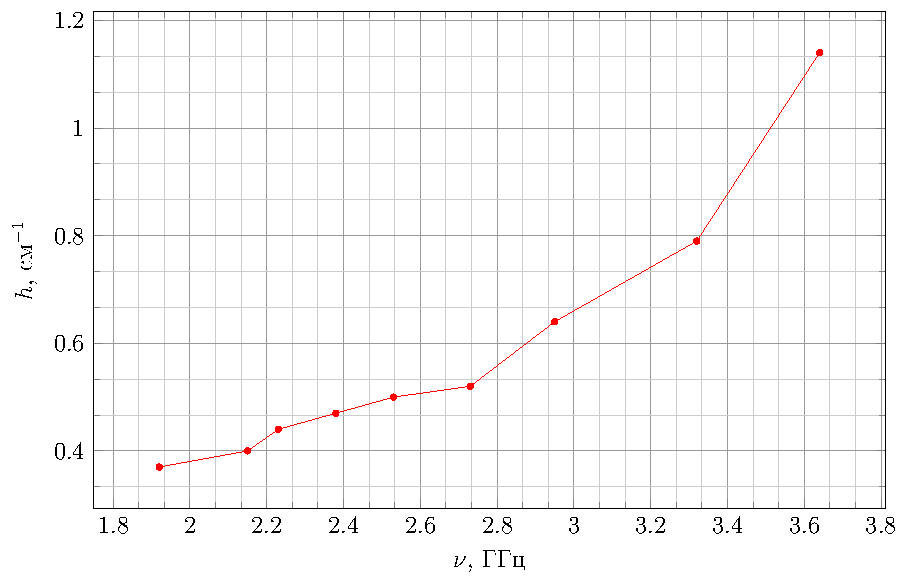
\includegraphics[width=0.8\linewidth]{plots/task1_2}
	\caption{дисперсионная характеристика гребенки 2 $l_1=8 \text{мм}$}
	\label{task1_2}
\end{figure}
\newpage
\subsection*{Задание 2}

\begin{table}[htbp]
	\centering
	\caption{гребенка 2, $l_2=8\text{мм}$, $\nu_1=2,179 \text{ГГц}$}
	\begin{tabular}{|l|r|r|r|r|r|r|r|r|r|}
		\hline
		I, мА & 27    & 13    & 4     & 15    & 25    & 30    & 20    & 5     & 10 \\
		\hline
		z, см & 8.33  & 9.33  & 10.5  & 11.3  & 12.3  & 12.67 & 13    & 13.8  & 17.5 \\
		\hline
	\end{tabular}%
	\label{tab:addlabel}%
\end{table}%

% Table generated by Excel2LaTeX from sheet 'задание2'
\begin{table}[htbp]
	\centering
	\caption{гребенка 2, $l_2=8\text{мм}$, $\nu_2=3,040 \text{ГГц}$}
	\begin{tabular}{|l|r|r|r|r|r|r|r|r|r|}
		\hline
		I, мА & 10    & 38    & 6     & 30    & 5     & 15    & 6     & 3     & 9 \\
		\hline
		z, см & 0.8   & 1.3   & 1.9   & 2.3   & 2.9   & 3.3   & 4.6   & 5.5   & 6.5 \\
		\hline
	\end{tabular}%
	\label{tab:addlabel}%
\end{table}%
\begin{figure}[H]
	\centering
	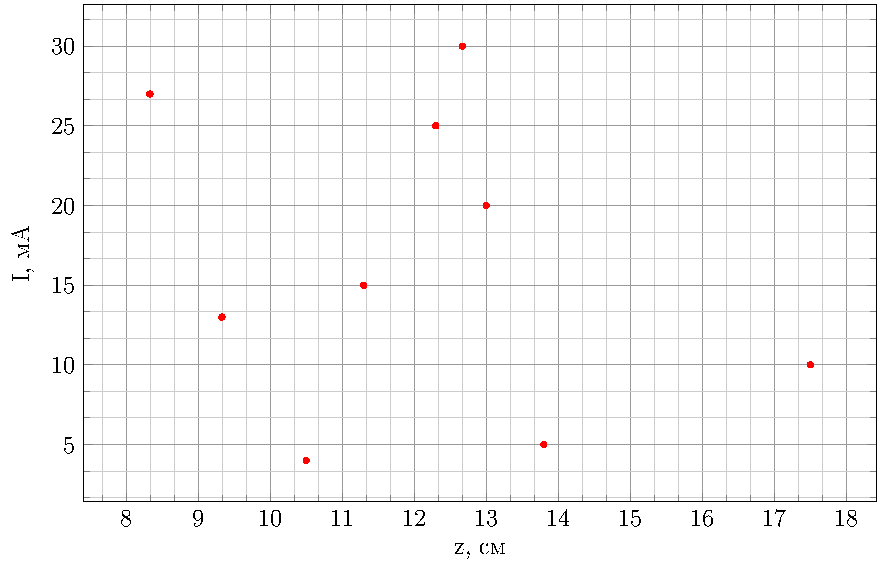
\includegraphics[width=0.8\linewidth]{plots/task2_1}
	\caption{Распределение поля вдоль системы, $\nu_1=2,179 \text{ГГц}$}
	\label{task2_1}
	\end{figure}

\begin{figure}[H]
	\centering
	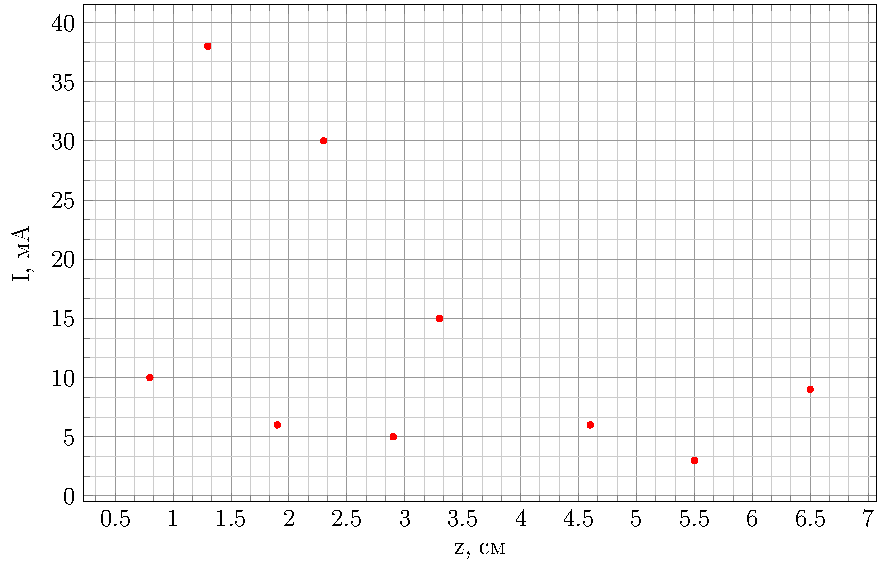
\includegraphics[width=0.8\linewidth]{plots/task2_2}
	\caption{Распределение поля вдоль системы, $\nu_2=3,040 \text{ГГц}$}
	\label{task2_2}
\end{figure}

При приближении к частоте запирания системы поверхностная волна, существующая в системе начинает быстро затухать с расстоянием. Таким образом интенсивность волны при удалении от источника начинает уменьшаться.
\end{document}